% ********** Приклад оформлення пояснювальної записки **********
% *********  до атестаційної роботи ступеня бакалавра **********


\documentclass{bachelor_thesis}

% Додаткові пакети вносіть у цей файл
%%%% У даний файл додавайте всі необхідні вам додаткові пакети, наприклад...


%%%% Диаграммы
%\usepackage{tikz}                      % !!! невідомий конфлікт з якимось іншим пакетом

% Пакети для кольорових текстів (необхідні для команди \todo)
%\usepackage{xcolor}                     % !!! невідомий конфлікт з якимось іншим пакетом
%\usepackage{colortbl}

\usepackage{euscript}   %ещё один красивый шрифт \EuScript

%%%% ...і таке інше

%\usepackage[normalem]{ulem} % для подчёркиваний uline
%\ULdepth = 0.16em % расстояние от линии до текста выше/ниже

% Додаткові визначення та перевизначення команд вносіть у цей файл
\input{02_redefinitions}

% Бюрократичні відомості про автора роботи
\input{03_data}


% Починаємо верстку документа
\begin{document}

\pagestyle{plain}
\setfontsize{14}

% Створюємо титульну сторінку
\begin{center}
	\begin{figure}[ht]
		\centering
		
\includegraphics[width=0.8\linewidth]{picture.png}	
	\end{figure}
	\hfill \break
	\footnotesize{Національний технічний університет України}\\ 
	\small{\textbf{«Київський політехнічний інститут»}}\\
	\hfill \break
	\normalsize{Фізико технічний інститут}\\
	\hfill \break
	\normalsize{Кафедра математичних методiв захисту iнформацiї}\\
	\hfill\break
	\LARGE{МЕТОДИ КРИПТОАНАЛІЗУ}\\
	\LARGE{КОМП’ЮТЕРНИЙ ПРАКТИКУМ №1}\\
	\hfill \break
	\Large{Баєсiвський пiдхiд в криптоаналiзi: побудова i
	дослiдження детермiнiстичної та стохастичної
	вирiшуючих функцiй}\\
    \hfill \break
    \hfill \break
	\hfill \break
	\hfill \break
	\hfill \break
	\hfill \break
	\end{center}
	
	
	\begin{flushright}
	Виконали:\\
	cтуденти групи ФІ-73\\
    Корж Нікіта\\
	Тафтай Анастасія\\
	\end{flushright}

	\begin{flushright}
		Перевірила:\\
		Ядуха Д. В.

		\hfill \break
		\hfill \break
	\end{flushright}
	
	\thispagestyle{empty}
	\begin{center} Київ 2021\end{center}

% Створюємо завдання
%\input{a01_specification}

% У даному костильному рішенні перші три сторінки (титул та завдання на 
% роботу) друкуються окремо від основної частини тез.
% Тому перша сторінка сформованого документу нумерується як четверта

% Створюємо анотації
%\setcounter{page}{4}
%\input{Chapters/a1_abstract}

% Створюємо зміст
%\pagenumbering{gobble}
%\tableofcontents
%\cleardoublepage
%\pagenumbering{arabic}
%\setcounter{page}{8}    %!!! -- продумати, як автоматизувати номер сторінки

% Створюємо перелік умовних позначень, скорочень і термінів
% Якщо цей розділ вам не потрібен, просто закоментуйте два наступних рядка
%\shortings
%\input{Chapters/a2_shortings}

% Створюємо вступ
%\intro
%\input{Chapters/a3_introduction}

% Додаємо глави
% Якщо ваша робота містить менше або більше глав - модифікуйте наступні 
% рядки відповідним чином
%!TEX root = ../thesis.tex

\newpage
    \section*{Мета роботи:}
    \qquad  Ознайомлення з принципами баєсiвського пiдходу в криптоаналiзi, побудова детермiнiстичної та стохастичної вирiшуючих функцiй для моделей схем шифрування та криптоаналiз моделей шифрiв за допомогою програмної реалiзацiї, зокрема здiйснення порiвняльного аналiзу вирiшуючих функцiй.

    \section*{Завдання}

    \begin{enumerate}
    \item  Ознайомитись з порядком виконання комп’ютерного практикуму та вiдповiдними вимогами до виконання роботи.
    \item Уважно прочитати необхiднi теоретичнi вiдомостi до комп’ютерного практикуму.
    \item Для заданого варiанта моделi шифру описати алгоритм побудови детермiнiстичної та стохастичної вирiшуючих функцiй. Створити репозиторiй в системi контролю версiй Git (бажано використовувати вебсервiс GitHub). Важливо:
    
    (а) репозиторiй створюється перед початком роботи над програмним кодом (якщо репозиторiй приватний, то перед початком роботи має бути надано доступ викладачу до даного репози- торiю);
        
    (б) весь процес створення програмного коду має бути вiдображений у вiдповiдних комiтах про- екту (для кожної атомарної змiни коду має бути власний комiт);
        
    (в) програмна реалiзацiя не допускається до захисту при недотриманнi вищевизначених вимог.
        
    \item Реалiзувати алгоритми програмно i подати результати побудови детермiнiстичної та стохастичної вирiшуючих функцiй у виглядi таблиць. Для цього необхiдно:
    
    (а) порахувати розподiли $P(C)$ та $P(M,C)$;
    
    (б) ґрунтуючись на цих розподiлах обчислити $P(M|C)$;
    
    (в) побудова оптимальних детермiнiстичної та стохастичної вирiшуючих функцiй зводиться до максимiзацiї $P(M|C)$.
    
    \item Обчислити середнi втрати, провести порiвняльний аналiз вирiшуючих функцiй.
    \end{enumerate}
    \begin{bf}
    Варіант завдання:
    \end{bf}
    16\\
\newpage
    \begin{center}
        \begin{Large}
            Хід роботи
        \end{Large}
    \end{center}
    
\section*{Опис алгоритму побудови детермiнiстичної та стохастичної вирiшуючих функцiй}
    
Для побудови детерміністичної функції використовувались значення $P(M|C)$ так, що $ \delta_{d}(C)  = index ~ \displaystyle\max_{M} P(M|C)$.
\\

Стохастична функція зберігає усі максимуми, тому вона будувалась так що в кожному рядку матриці на місцях максимальних елементів вона дорівнювала $(1 ~~ / $ кількість максмимальних елементів у рядку$)$, а на місцях не максимальних елементів дорівнювала нулю.
    
\newpage

\textbf{Таблиця $P(M|C)$ для 16 варіанту }
\begin{figure}[h!]
\center{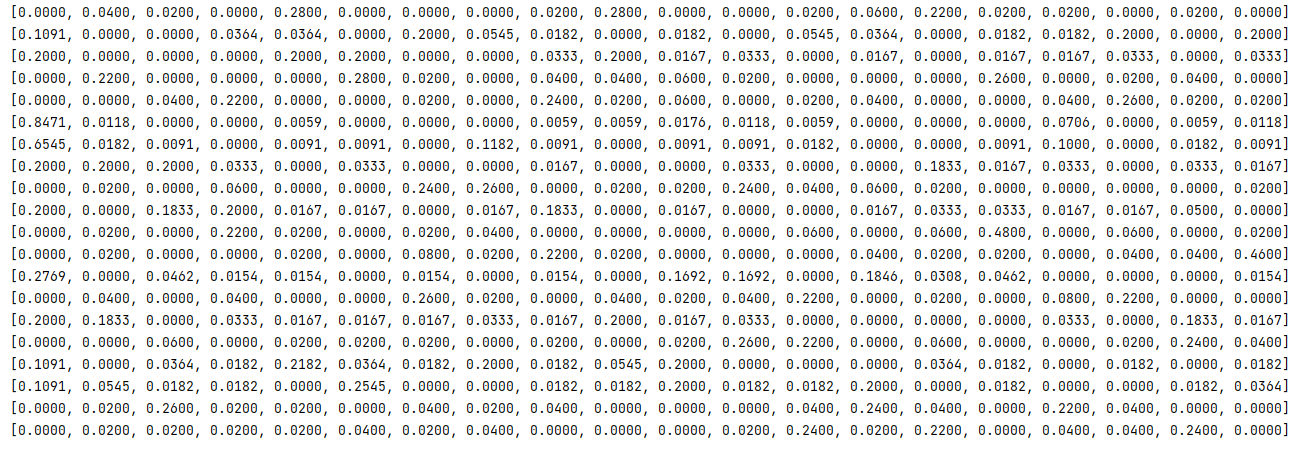
\includegraphics[scale=0.5]{1.png}}
\label{fig:image}
\end{figure}
    
\textbf{Таблиця $P(M|C)$ для 6 варіанту } 
\begin{figure}[h!]
\center{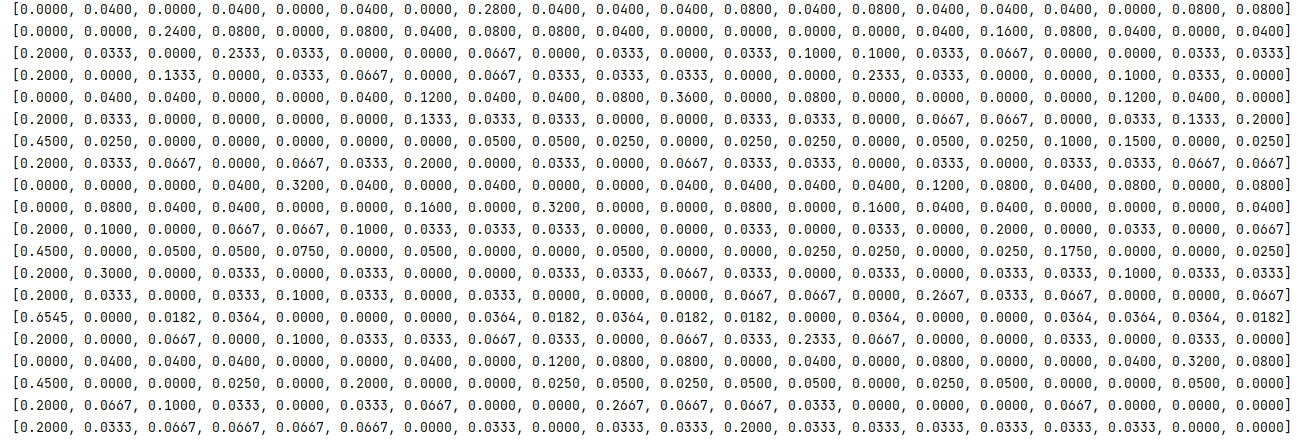
\includegraphics[scale=0.5]{2.png}}
\label{fig:image}
\end{figure}  
 
\newpage

\textbf{Знайденi детермiнiстична та стохастична функцiї у виглядi таблиць для 16 варіанту}
\\

Детерміністична функція:\\
\begin{figure}[h!]
\center{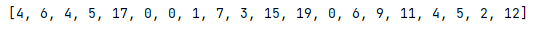
\includegraphics[scale=0.5]{3.png}}
\label{fig:image}
\end{figure}  
    
Стохастична функція:\\
\begin{figure}[h!]
\center{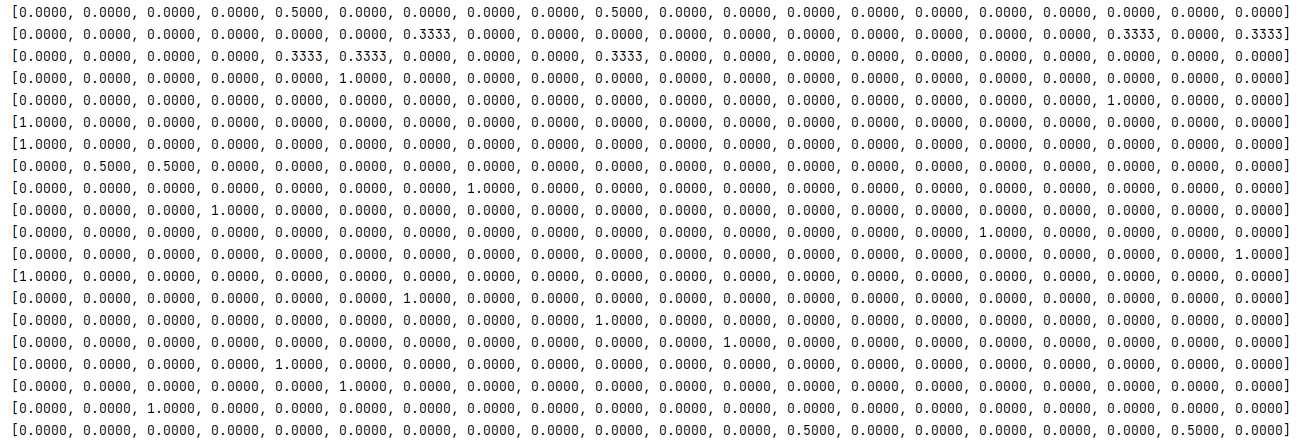
\includegraphics[scale=0.5]{4.png}}
\label{fig:image}
\end{figure}    

\newpage
\textbf{Знайденi детермiнiстична та стохастична функцiї у виглядi таблиць для 6 варіанту}
\\

Детерміністична функція:\\
\begin{figure}[h!]
\center{
\includegraphics[scale=0.5]{6.png}}
\label{fig:image}
\end{figure}      

Стохастична функція:\\
\begin{figure}[h!]
\center{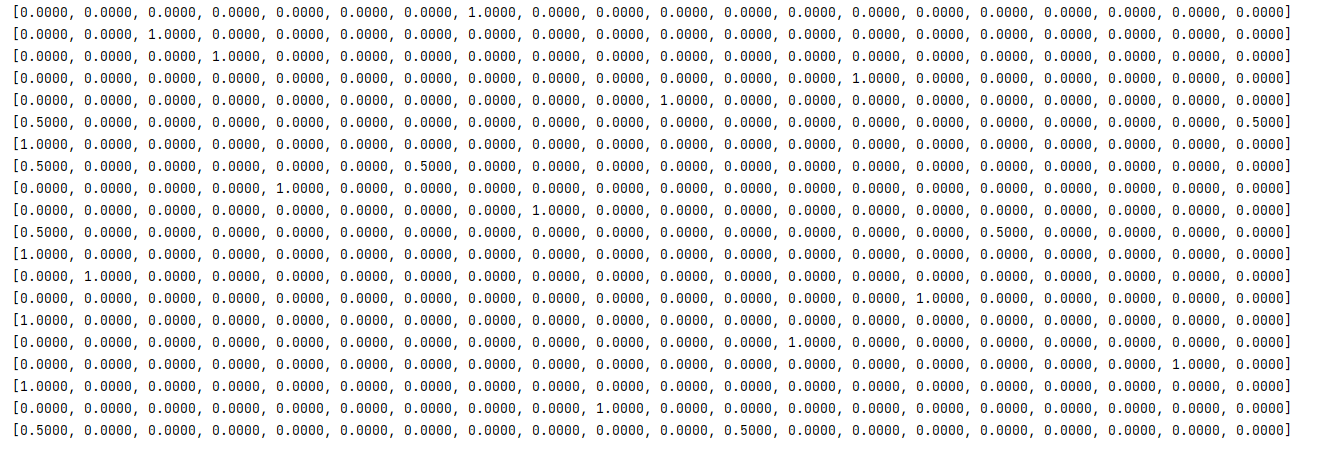
\includegraphics[scale=0.5]{5.png}}
\label{fig:image}
\end{figure}      


\newpage
\textbf{Cереднi втрати для вирiшуючих функцiй для 16 варіанту}
\\

Для детерміністичної вирішуючої функції : \textbf{0.6232000000000001}
\\

Для стохастичної вирішуючої функції : \textbf{0.6232000000000001} 
\\
    
\textbf{Cереднi втрати для вирiшуючих функцiй для 6 варіанту}
\\
   
Для детерміністичної вирішуючої функції: \textbf{0.6703999999999998} 
\\

Для стохастичної вирішуючої функції: \textbf{0.6703999999999998} 
\\


\textbf{Опис труднощiв, що виникали при виконаннi комп’ютерного практикуму, та шляхи їх розв’язання:}
\\

Під час виконання лабораторної роботи виникли невеликі труднощі з побудовою ймовірностей та розумінням, як саме необхідно будувати стохастичну вирішуючу функцію, а також була проблема в похибці при операціях з числами з плаваючою точкою.
\\  

\textbf{Порівняльний аналіз детерміністичної і стохастичної вирішуючих функцій}
\\

При виконанні даної роботи було побудовано детерміністичну і стохастичку вирішувані функції, а також було пораховано середні втрати для детермінстичної і стохастичної вирішуваних функцій. Після виконання роботи був проведений аналіз роботи цих функцій і був зроблений висновок, що обидві функції є однаково ефективними, оскільки середні втрати для обох функцій однакові.
%\input{Chapters/c2_chapter_02}
%\input{Chapters/c3_chapter_03}


% Створюємо висновки
\conclusions
%!TEX root = ../thesis.tex
% створюємо Висновки до всієї роботи

 Під час роботи ми ознайомилися з принципами баєсiвського пiдходу в криптоаналiзi. Побудували детермiнiстичну та стохастичну вирiшуючі функцiї, а також були пораховані середні втрати як для детерміністичної вирішуючої функції, так і для стохастичної вирішуючої функції. На основі результатів виконання роботи, було проведено аналіз заданих вирішуючих функцій і було зроблено висновок, що обидві функції є однаково ефективними.  

% Додаємо бібліографію
% Якщо ви володієте магією bibtex-у, використовуйте її та модифікуйте файл 
% з бібліографією відповідним чином
%\input{Chapters/w2_bibliography}

%\bibliographystyle{ugost2008}
%\bibliography{thesis}

% Створюємо додатки (дивись у файли додатків для необхідних пояснень)
% Якщо ви маєте меншу або більшу кількість додатків, модифікуйте наступні 
% рядки відповідним чином
% Якщо ви не маєте додатків, просто закоментуйте наступні рядки
%\input{Chapters/z1_appendix_A}
%\input{Chapters/z2_appendix_B}


% Нарешті
\end{document}